Queremos observar que tan bueno es el algoritmo propuesto en la práctica.
Para estudiar el desempeño del algoritmo utilizaremos las familias \textbf{Random} y \textbf{Gimnasios por grupos}. 

Nos interesa particularmente si el algoritmo logra sortear el principal problema que tiene búsqueda local que es justamente, la localidad de las soluciones.

La idea, además, es tratar de encontrar la configuración de Tabú Search ideal para que en promedio el algoritmo resuelva la mayoría de los casos eficientemente. Para lograr esto, se experimenta variando distintos parametros del algoritmo para cada entrada.

Los parámetros de estudio serán:

\begin{itemize}
\item  \textbf{Cantidad de iteraciones}: Tenemos que observar en promedio, cuantas iteraciones conviene tomar para obtener un buen resutado.
\item \textbf{Tenor tabú}: Tenemos que observar que sucede al aumentar el tenor tabú, y hasta cuanto es conveniente hacerlo para obtener un buen resultado.
\end{itemize}

Para realizar los tests se generaron dos rangos de instancias:

Para realizar los tests se tomaron dos rangos de tamaños:
\begin{itemize}
\item Rango 1: 5 a 15 elementos (pokeparadas + gimnasios)
\item Rango 2: 20 a 100 en intervalos de 10 elementos.
\end{itemize}

Para el Rango 1 se tomaron 5$\ast n$ instancias siendo $n$ el tamaño de entrada (pokeparadas + gimnasios) y para el Rango 2 se tomó el 50\% del tamaño de la entrada. El Rango 2 es más pequeño que en el punto tres, ya que tabú search requiere mucho más tiempo de resolución y por lo tanto se decidió tomar tamaños de hasta 100 elementos pero discretizar mejor.\\

Todas las distancias y tiempos de las instancias de un mismo tamaño son promediadas para obtener porcentajes de mejora con respecto a la solucion promedio golosa y poder comparar los resultados con la solución exacta para el Rango 1.\\

\subsubsection*{Tenor}

Comenzaremos analizando este parámetro para las familias \textbf{Random} y \textbf{Grupos de gimnasios}.
Nos interesaba entender cual sería el comportamiento del algoritmo al aumentar el tenor tabú.

Dado que la lista tabú almacena aristas, tenemos que determinar un porcentaje de aristas limite para el tamaño de esta lista. Aquellas almacenadas serán marcadas como tabú y por lo tanto atributos no deseables en una solución.
Por lo tanto Sea $C$ = $m+n$ = pokeparadas + gimnasios, el tamaño de la entrada, el mapa conformado por estos elementos tendra todas las aristas posibles, que son en total, $\frac{C \ast C-1}{2}$, entonces la cantidad de aristas que podremos marcar como tabú estará acotado por ese valor.\\
Para este test decidimos probar con dos rangos de valores para el tenor, 1\% a 5\% y 10\% a 50\% de la cantidad de aristas totales en el mapa.

Por lo tanto para realizar los tests, se configuró el algoritmo tabú de la siguiente manera:

\begin{itemize}
\item Tenor: variable desde C $\ast$ 0.01 hasta C $\ast$ 0.05 en intervalos de 0.01 y C $\ast$ 0.1 hasta C $\ast$ 0.5 en intervalos de 0.1
\item Criterio de parada: iteraciones límite $T$ = C $\ast$ 0.10 si C >= 20, si no C.
\end{itemize}

El criterio de parada se eligió inicialmente en \textbf{cantidad de iteraciones límite} ya que con el segundo criterio de parada, \textbf{Repeticiones límite sin mejora} se requería bastante más tiempo de corrida. 

Entendemos que lo mejor hubiese sido probar con ambos criterios, aunque desestimamos que se hubiesen obtenido resultados diferentes, ya que el segundo criterio en si, como veremos luego, tiene una muy buena performance para valores de tenor pequeños.\\

Veamos los gráficos para los resultados de ambas familias y ambos rangos de entada.
\\\\

\begin{figure}[h] 
 \centering
  \subfloat[Rango 1: Familia Random]{
    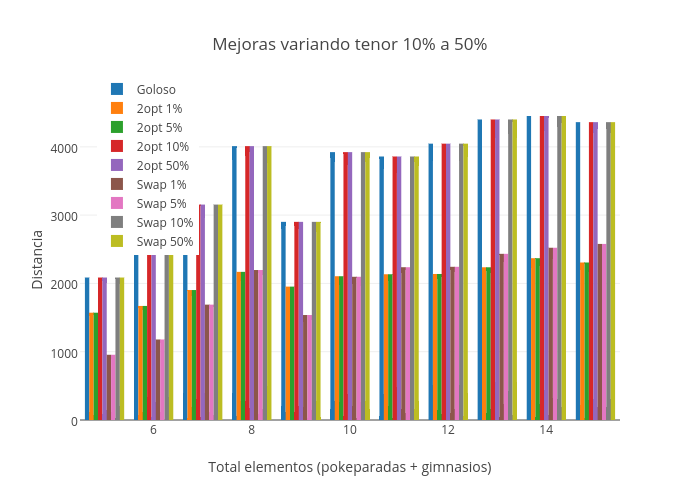
\includegraphics[width=0.45\textwidth]{./EJ4/tenorRandom15c.png}}
       \label{fig:randomDist1}
  \subfloat[Rango 2: Familia Random]{
    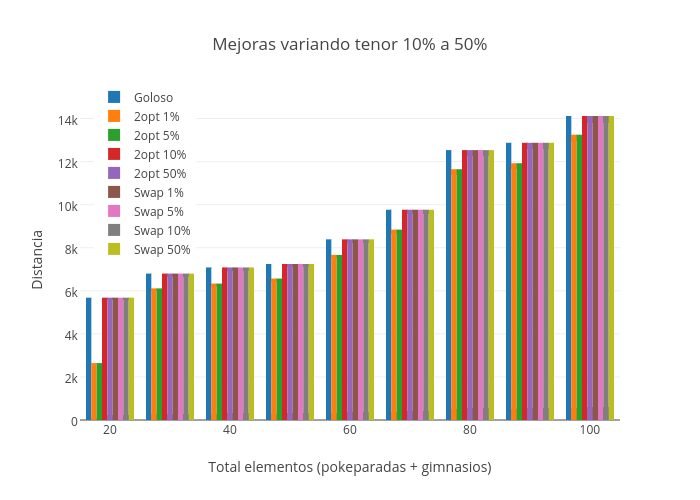
\includegraphics[width=0.45\textwidth]{./EJ4/tenorRandom100.png}}
    \label{fig:randomMejora1}
\end{figure}

\begin{figure}[h] 
 \centering
  \subfloat[Rango 1: Familia Grupos de gimnasios]{
    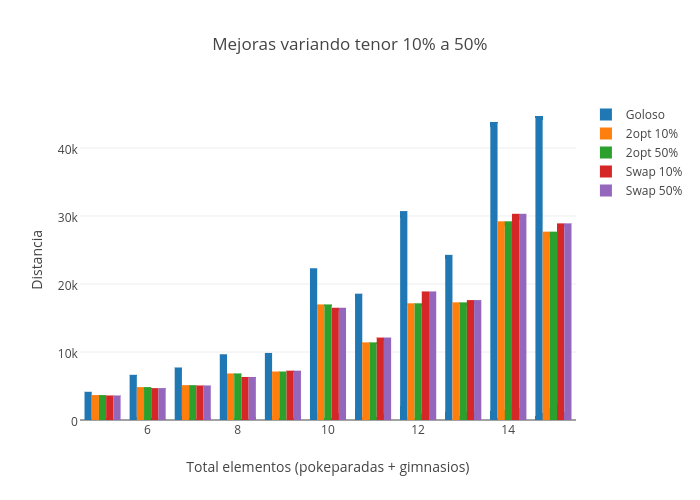
\includegraphics[width=0.45\textwidth]{./EJ4/tenorFamilia15c.png}}
       \label{fig:randomDist1}
  \subfloat[Rango 2: Familia Grupos de gimnasios]{
    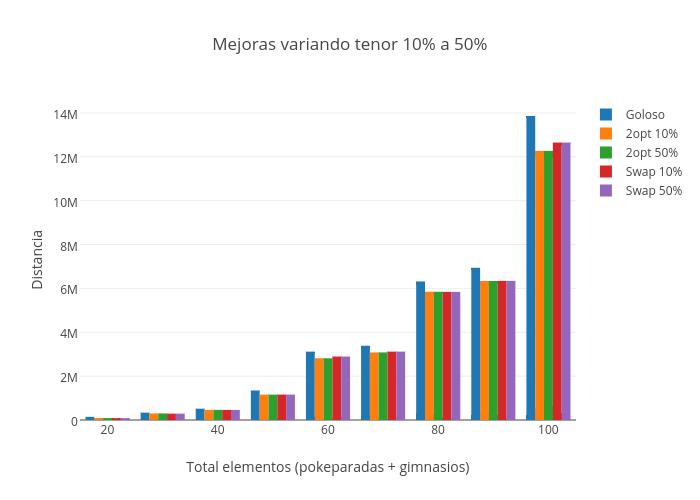
\includegraphics[width=0.45\textwidth]{./EJ4/tenorFamilia100.png}}
    \label{fig:randomMejora1}
\end{figure}

En los gráficos se pueden ver 9 columnas de distancias:

\begin{enumerate}
\item Goloso
\item Tabú - 2opt con tenor 1\%
\item Tabú - 2opt con tenor 5\%
\item Tabú - 2opt con tenor 10\%
\item Tabú - 2opt con tenor 50\%
\item Tabú - Swap con tenor 1\%
\item Tabú - Swap con tenor 5\%
\item Tabú - Swap con tenor 10\%
\item Tabú - Swap con tenor 50\%
\end{enumerate}

Como puede observarse, tener valores grandes de tenor no beneficia al resultado del algoritmo, más bien, todo lo contrario. Esto puede relacionarse con que valores grandes de tenor implica ser más restrictivo y darle al algoritmo mucha memoria tabú, y esto puede perjudicar las regiones que el algoritmo puede checkear. Por lo tanto conviene siempre tener valores pequeños del tenor, para ser restrictivos en regiones pequeñas y permitir al algoritmo alejarse hacia soluciones que tengan aristas que hayan sido tabú pero que hayan sido reemplazadas con nuevas aristas, lo que puede llevar a descubrir soluciones nuevas, es decir recorridos nuevos, que sean mejores.\\

Por lo tanto determinamos que tomare entre un 1\% y un 10\% de las aristas totales es un buen valor para el tenor. En lo que sigue, trabajaremos con un 5\%.

\subsection*{Iteraciones límite vs. Repeticiones límite sin mejora}

La cantidad de iteraciones Límite fue testeó desde el 10\% al 50\% del tamaño de la entrada y la cantidad de repeticiones límite sin mejora desde 1 hasta 10.\\
En principio, a la hora de realizar el test, la cantidad de iteraciones límite para obtener un valor que fuera de calidad era desconocido, así que lo que se verá en los gráficos refleja es una consecuencia de la cantidad de iteraciones límite elegida.

Veamos que sucedió para ambas familias

\begin{figure}[h] 
 \centering
  \subfloat[Distancias: Familia Random]{
    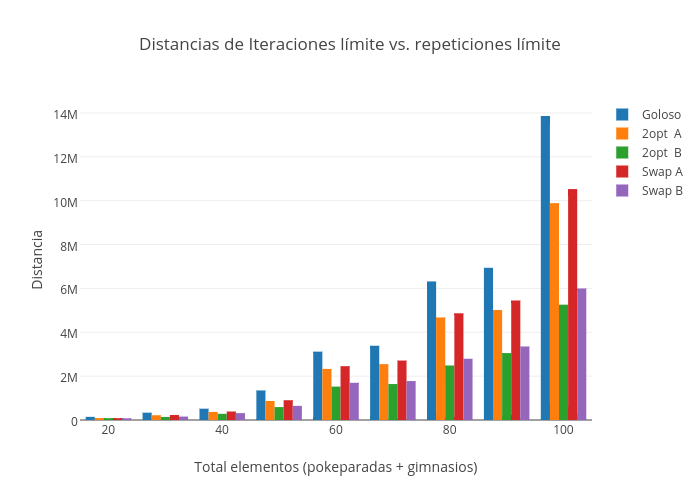
\includegraphics[width=0.45\textwidth]{./EJ4/criteriosDistanciasFamilia100.png}}
       \label{fig:randomDist1}
  \subfloat[Tiempos: Familia Random]{
    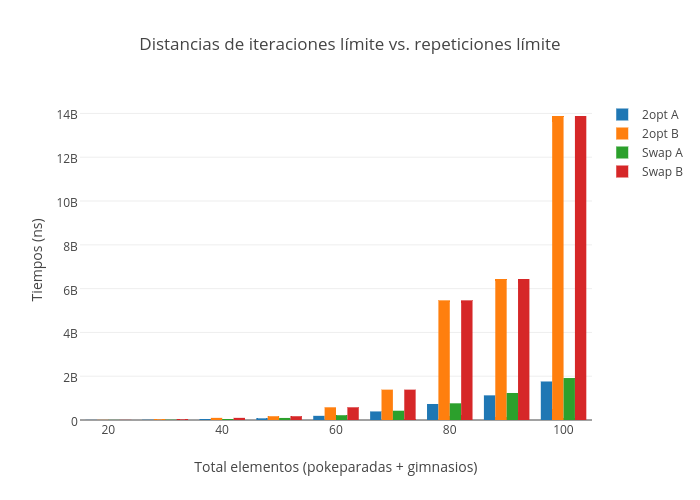
\includegraphics[width=0.45\textwidth]{./EJ4/criteriosTiemposRandom100.png}}
    \label{fig:randomMejora1}
\end{figure}

\begin{figure}[h] 
 \centering
  \subfloat[Distancias: Familia Random]{
    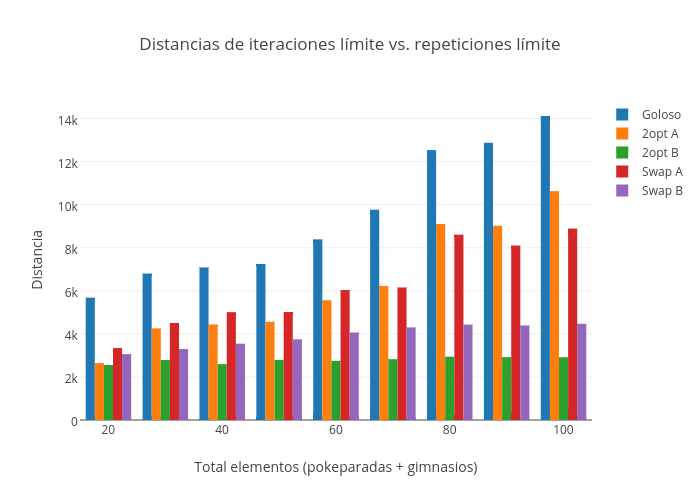
\includegraphics[width=0.45\textwidth]{./EJ4/criteriosDistanciasRandom100.png}}
       \label{fig:randomDist1}
  \subfloat[Tiempos: Familia Random]{
    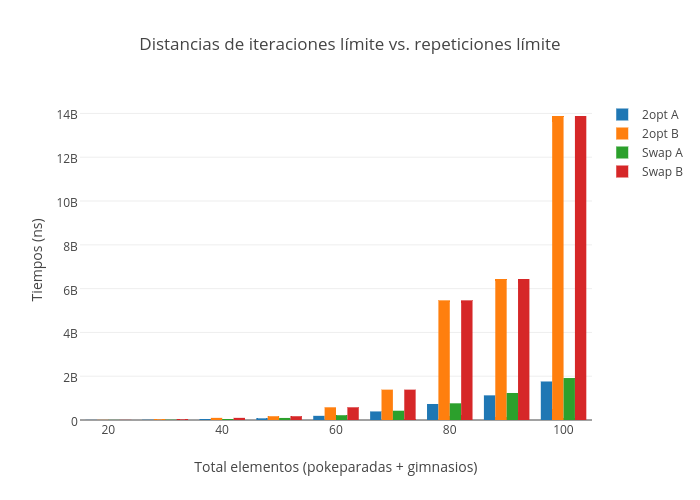
\includegraphics[width=0.45\textwidth]{./EJ4/criteriosTiemposRandom100.png}}
    \label{fig:randomMejora1}
\end{figure}

En los gráficos se pueden ver 5 columnas:

\begin{enumerate}
\item Goloso
\item Tabú - 2opt iteraciones límite.
\item Tabú - 2opt repeticiones límite
\item Tabú - Swap iteraciones límite
\item Tabú - Swap repeticiones límite
\end{enumerate}

Puede verse claramente como repeticiones límite gana en ambas versiones de tabú search (2opt y Swap), aunque con un costo considerable de tiempo. Con iteraciones límite no se obtuvo una solución tan buena (es en general un 50\% , 60\% o 70\% peor, como es el caso de 2opt) aunque el resultado se obtiene en la mitad de tiempo. Para obtener un resultado mejor usando cantidad de iteraciones límite, deberá iterarse hasta encontrar un valor que haga que el resultado no mejore. 

Una forma trivial de saber cuantas iteraciones hay que tomar, sería contando la cantidad de iteraciones que hace el algoritmo usando repeticiones límite para varios casos del mismo tamaño y promediando los mismos. Si este valor puede compararse con algún parámetro, como podría ser un porcentaje del tamaño de entrada, podrían esablecerse rangos de valores donde vaya disminuyendo la distancia pero tenga que resignarse tiempo. De cualquier manera es una tarea que requiere mucho tiempo.\\

Siendo que usando el criterio de corte de repeticiones límite, tabú-2opt es el que mejores soluciones brinda para ambas familias, para el caso de el criterio de corte por repetición podemos ver claramente que para valores grandes en la familia Random es tabú-Swap quien tiene los mejores resultados. Podemos ver esto en los siguientes gráficos.

Veamos esto para 100 elementos.\\

\begin{figure}[h] 
 \centering
  \subfloat[Distancias Random]{
    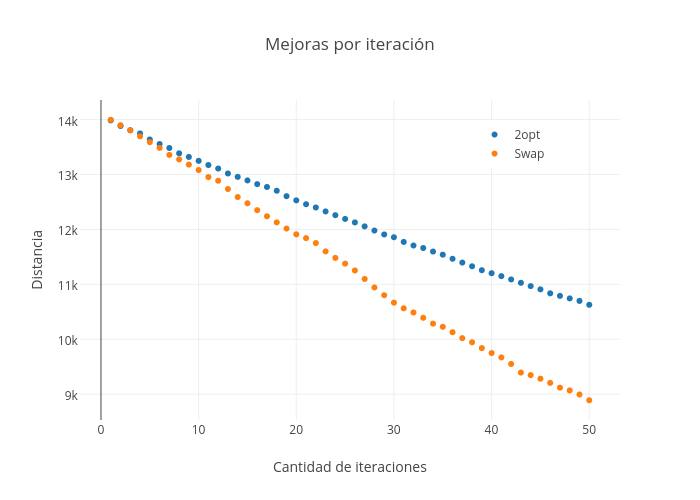
\includegraphics[width=0.45\textwidth]{./EJ4/mejorasDistRandom100.png}}
       \label{fig:randomDist1}
  \subfloat[Distancias Grupos de gimnasios]{
    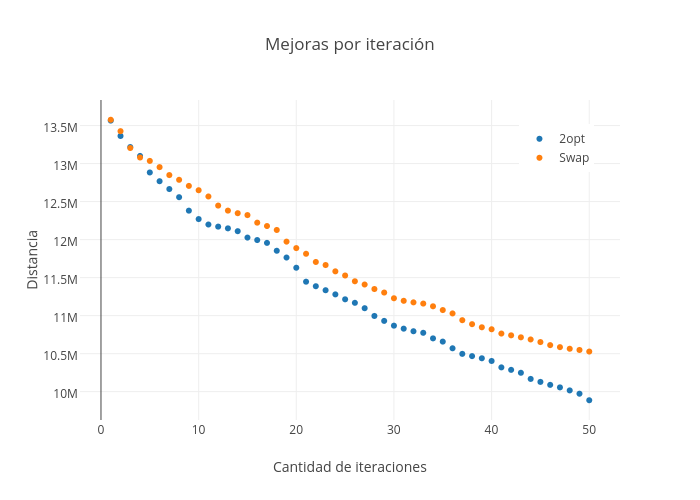
\includegraphics[width=0.45\textwidth]{./EJ4/mejorasDistFamilia100.png}}
    \label{fig:randomMejora1}
\end{figure}

\newpage

Mientras que para Grupos de gimnasios tabú-2opt es la mejor opción con cualquier criterio de corte, para la familia Random, si se utiliza el criterio de corte por iteraciones límite puede verse que la mayor ventaja se dá utilizando tabú-Swap.
Dado que la familia Random es muy general en cuanto a instancias posibles, y que en la mayoría de los casos 2opt fué el que mejores resultados dió, no sabemos como explicar porque sucede esto. 
Creemos igualmente que si realizan más iteraciones,  tabú-2opt se verá beneficado de ello y tal como sucede en los otros casos.\\

Claramente es difícil determinar un buen valor de iteraciones límite prematuramente, por lo tanto si se quiere estar seguro de obtener un muy buen resultado, cantidad de repeticiones límite es el mejor aliado.

Veamos los siguientes gráficos que muestram que utilizando un valor de 2 como repeticiones límite es suficiente para la condición de corte.

\begin{figure}[h] 
 \centering
  \subfloat[Distancias Random]{
    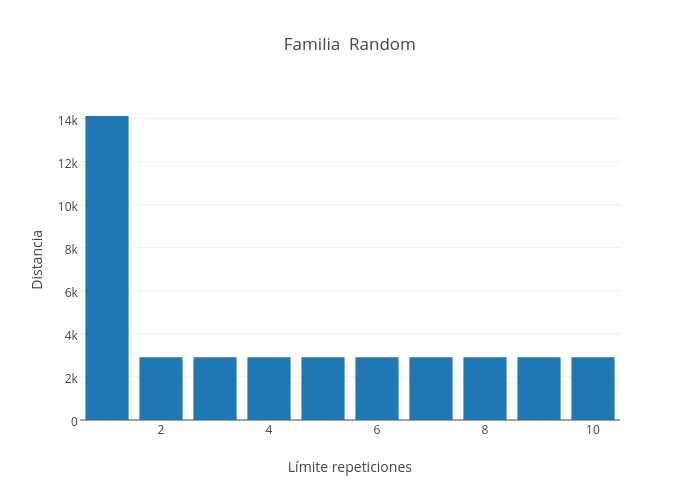
\includegraphics[width=0.45\textwidth]{./EJ4/cantRepRandom100.png}}
       \label{fig:randomDist1}
  \subfloat[Distancias Grupos de gimnasios]{
    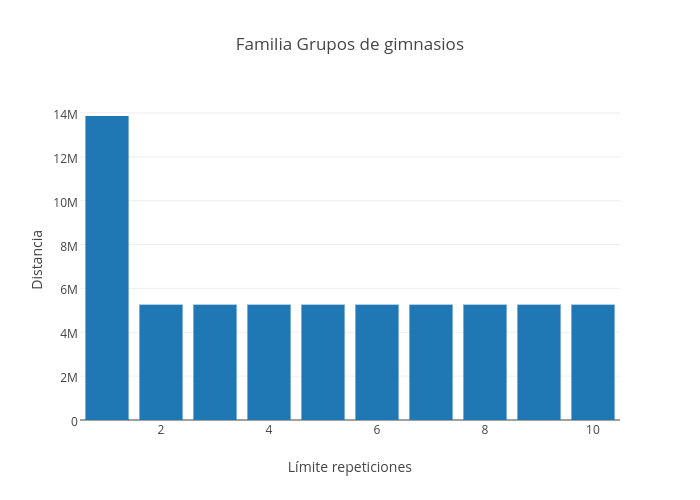
\includegraphics[width=0.45\textwidth]{./EJ4/cantRepFamilia100.png}}
    \label{fig:randomMejora1}
\end{figure}

Por lo tanto, la mejor configuración es usar cantidad de repeticiones límite igual a dos (aunque a costa del tiempo) y un valor de tenor igual al 5\% del tamaño de entrada.

El problema del tiempo requerido para correr tabú search fué una constante durante toda la experimentación, hasta el final. Para poder mejorar este inconveniente y dado que los algoritmos fueron implementados utilizando el lenguaje C++, se recurrió a compilar los algoritmos utilizando el flag de optimización O3 que fué determinante a la hora de acelerar la corrida de los tests, que de otra forma nos hubiera limitado a promediar menos o generar casos de tests más pequeños en cuanto a tamaño.\\

\subsection*{Comparación con solución de búsqueda local y solución exacta}

En este apartado nos interesa comparar las mejores soluciones de tabú search para cada familia contra lo mejor encontrado por la búsqueda local y los tiempso requeridos para ello. Además, para el Rango 1 podremos saber que tan cerca se encuentra la solución tabú midiendo el error relativo.\\

\subsubsection*{Error relativo Random}

\begin{figure}[h] 
 \centering
  \subfloat[Error relativo Tabú 2opt vs. Búsqueda local 2opt]{
    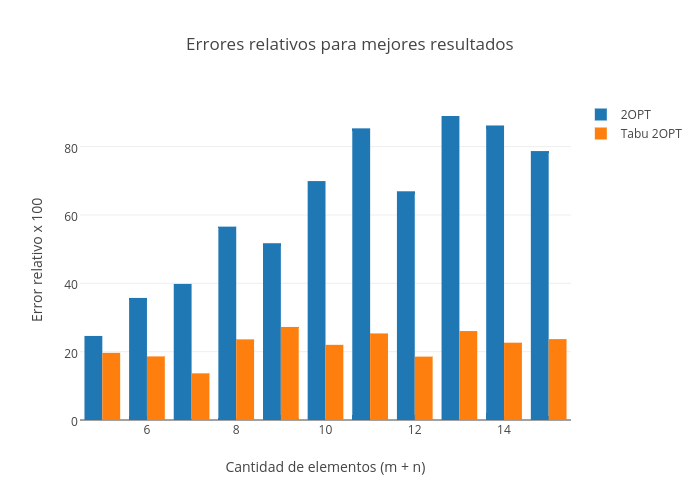
\includegraphics[width=0.45\textwidth]{./EJ4/errorRelativoTabuRandom.png}}
       \label{fig:randomDist1}
  \subfloat[Tiempos Tabú 2opt vs. Búsqueda local 2opt]{
    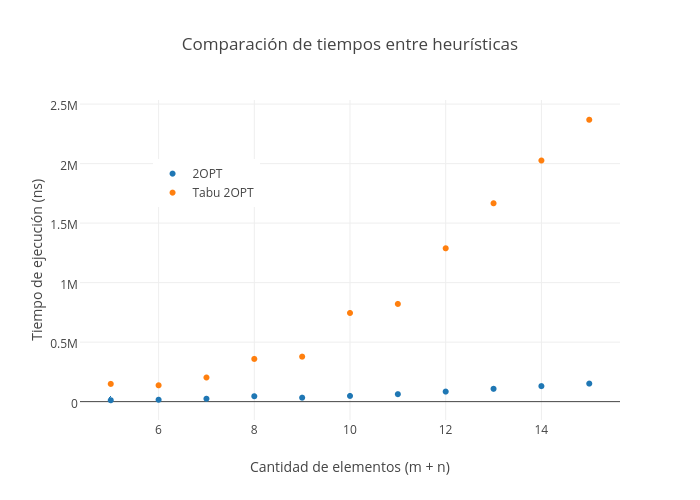
\includegraphics[width=0.45\textwidth]{./EJ4/tiempoChicoRandom.png}}
    \label{fig:randomMejora1}
\end{figure}

Podemos notar que para casos pequeños, es conveniente aplicar tabú search en la familia Grupos de gimnasios, donde  se obtienen errores cercanos al 20\% en comparación a los errores de la búsqueda local, que están en su mayoria por encima del 40\%. Esto aún considerando los tiempos necesarios de corrida para obtener estas soluciones, que son bastante superiores a los requeridos por la búsqueda local. 

Sabemos por lo que hemos estudiado hasta el momento, que las soluciones obtenidas por el algoritmo goloso para la familia por grupos puede ser muy mala, y en casos pequeños siempre se puede mejorar mucho una solución y más utilizando un algoritmo que intenta escapar de los mínimos locales como tabú search.\\

\subsubsection*{Error relativo Grupos de familia}

\begin{figure}[h] 
 \centering
  \subfloat[Error relativo Tabú 2opt vs. Búsqueda local 2opt]{
    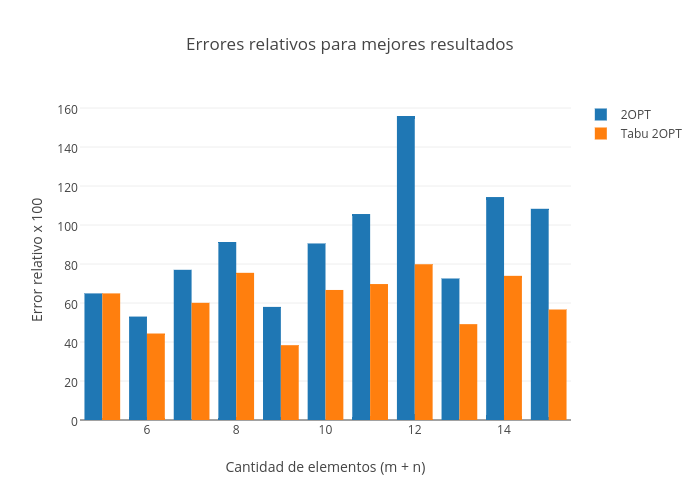
\includegraphics[width=0.45\textwidth]{./EJ4/errorRelativoTabuFamilia.png}}
       \label{fig:randomDist1}
  \subfloat[Tiempos Tabú 2opt vs. Búsqueda local 2opt]{
    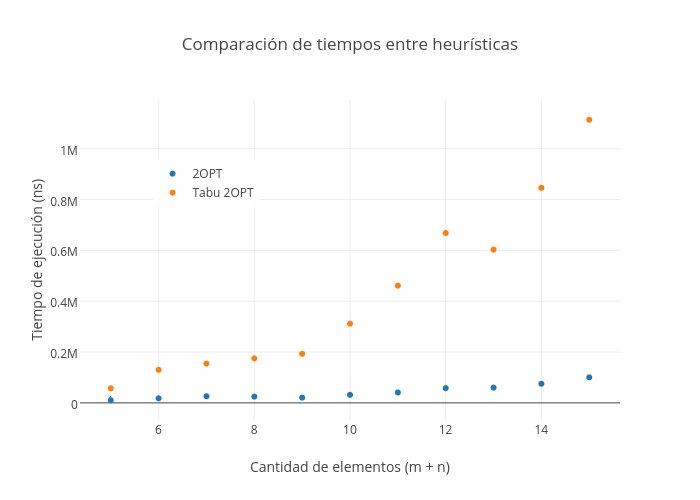
\includegraphics[width=0.45\textwidth]{./EJ4/tiempoChicoFamilia.png}}
    \label{fig:randomMejora1}
\end{figure}

Dado que la familia Random está conformada por casos más generales, no siempre todas las soluciones que el algoritmo goloso encuentra para cada ejemplo dentro de un tamaño pueden ser malas. Por lo tanto los errores son más variables y no una hay una diferencia muy marcada entre tabú search y la búsqueda local, aunque si puede verse que tabú siempre es mejor, con errores que no superan el 80\% mientras que para la mayoria de los casos la búsqueda local si se supera este valor.\\

En general puede verse que ninguna solución alcanza la distancia óptima para estos tamaños. Encontrar este valor puede ser muy difícil incluso para tamaños pequeños, ya que si existen muchas combinacioens de soluciones válidas, tabú search podría tener que recorrerlas todas antes de llegar a la solución óptima.\\

\subsubsection*{Porcentajes de mejora para casos grandes}

Para los casos grandes solo podemos ver que tanto se mejora la solución con respecto al goloso, ya que es practicamente imposible correr backtracking sobre tamaños superios a 15 aristas teniendo que promediar instancias en tiempos razonables.\\

Para poder realizar comparaciones, se corrieron las mismas instancias del Rango 2 de este punto con los algoritmos de búsqueda local que mejores resultados obtuvieron en el ejercicio tres.\\

\begin{figure}[h] 
 \centering
  \subfloat[Porcentaje de mejora Tabú 2opt vs. Búsqueda local 2opt]{
    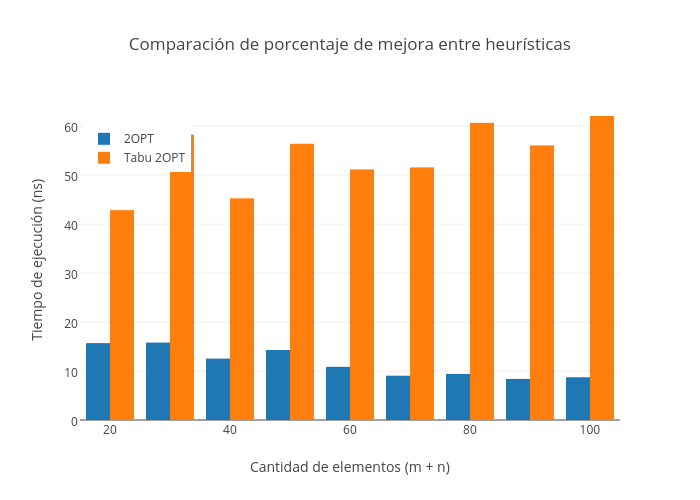
\includegraphics[width=0.45\textwidth]{./EJ4/mejoraFamilia.png}}
       \label{fig:randomDist1}
  \subfloat[Tiempos Tabú 2opt vs. Búsqueda local 2opt]{
    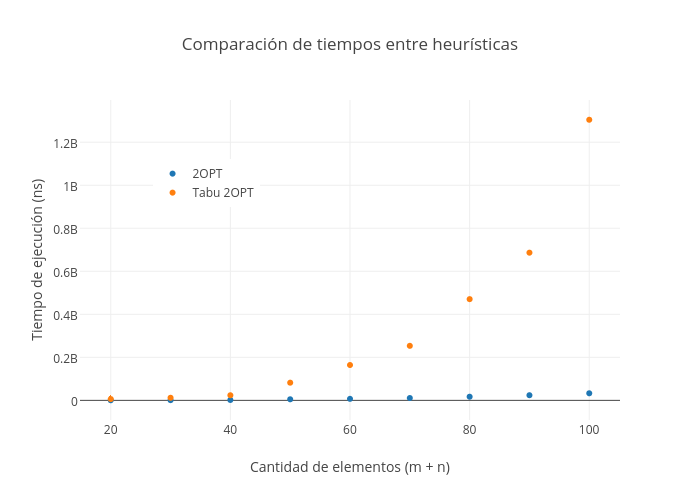
\includegraphics[width=0.45\textwidth]{./EJ4/tiempoGrandeFamilia.png}}
    \label{fig:randomMejora1}
\end{figure}

\begin{figure}[h] 
 \centering
  \subfloat[Porcentaje de mejora Tabú 2opt vs. Búsqueda local 2opt]{
    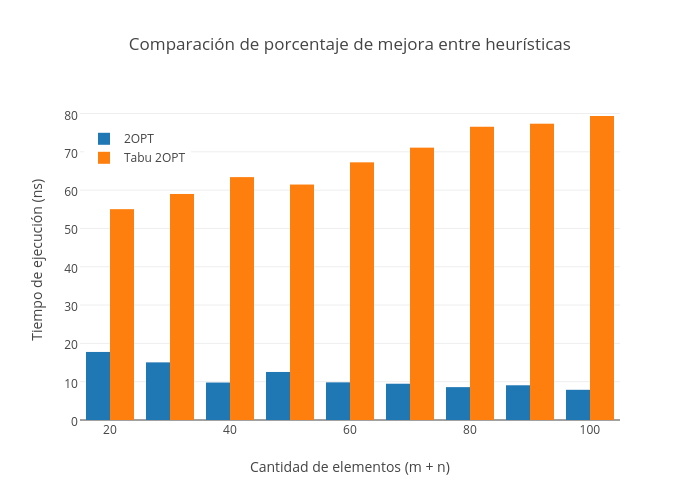
\includegraphics[width=0.45\textwidth]{./EJ4/mejoraRandom.png}}
       \label{fig:randomDist1}
  \subfloat[Tiempos Tabú 2opt vs. Búsqueda local 2opt]{
    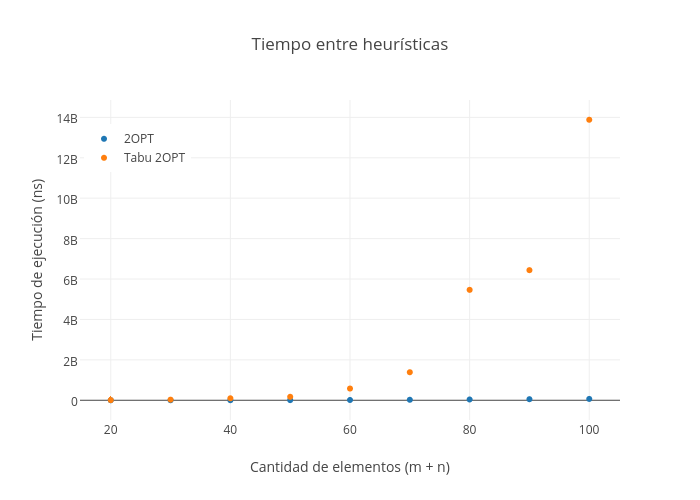
\includegraphics[width=0.45\textwidth]{./EJ4/tiempoGrandeRandom.png}}
    \label{fig:randomMejora1}
\end{figure}

Sin lugar a dudas, para instancias grandes, conviene utilizar tabú search, aunque deba pagarse un alto coste temporal. Puede verse que el porcentaje de mejora para ambas familias supera el 50\% mientras que con la búsqueda local se obtiene un porcentaje de mejora inferior al 20\% en ambos casos. Con lo cual, parece confirmarse que cuanto más grande la instancia, más local quedan las soluciones obtenidas por una heurística de búsqueda local, mientras que tabú search encuentra mejores soluciones analizando muchas más vecindades.

